% !TeX program = xelatex
\ifdefined\BookMaster\else
\documentclass[11pt,oneside]{article}
% !TeX program = xelatex
\usepackage[b5paper,left=22mm,right=22mm,top=20mm,bottom=22mm,footskip=11mm]{geometry}
\usepackage{fontspec}
\setmainfont{TeX Gyre Termes}
\setsansfont{TeX Gyre Heros}
\usepackage{amsmath,amssymb,mathtools,amsthm}
\renewcommand{\cdots}{\mathinner{\cdotp\cdotp\cdotp}}
\usepackage{graphicx,adjustbox,array,booktabs,longtable,multirow,enumitem,changepage,needspace}
\usepackage[table]{xcolor}
\usepackage{fancyhdr}
\raggedbottom
\interfootnotelinepenalty=10000
\newcommand{\BookFootnote}[2]{\begingroup\renewcommand{\thefootnote}{\fnsymbol{footnote}}\footnote[#1]{#2}\endgroup}
\newcommand{\BookFootnoteMark}[1]{\begingroup\renewcommand{\thefootnote}{\fnsymbol{footnote}}\footnotemark[#1]\endgroup}
\newcommand{\BookFootnoteText}[2]{\begingroup\renewcommand{\thefootnote}{\fnsymbol{footnote}}\footnotetext[#1]{#2}\endgroup}
\newenvironment{BookFloat}[1]{\par\addvspace{.6\baselineskip}\noindent\def\BookFloatID{#1}\begin{minipage}{\linewidth}\phantomsection\label{bookfloat:#1:start}}{\phantomsection\label{bookfloat:\BookFloatID:end}\end{minipage}\par\addvspace{.6\baselineskip}}

\usepackage[unicode,hidelinks]{hyperref}
\pagestyle{fancy}
\fancyhf{}
\newcommand{\BookFooter}{}
\fancyfoot[L]{\parbox[b]{\dimexpr\textwidth-15mm}{\footnotesize\BookFooter}}
\fancyfoot[R]{\footnotesize\thepage}
\renewcommand{\headrulewidth}{0pt}
\renewcommand{\footrulewidth}{0pt}
\setlength{\parindent}{0pt}
\setlength{\parskip}{0.2em}
\setlength{\emergencystretch}{3em}
\setlist{nosep,leftmargin=1.7em,labelsep=.65em}
\newif\ifBookNarrative
\BookNarrativetrue
\newenvironment{BookBody}{\setlength{\parindent}{0pt}}{}
\newcommand{\BookStatement}[1]{\par\addvspace{.6\baselineskip}\noindent #1\enspace\ignorespaces}
\newcommand{\BookLabel}[1]{\par\addvspace{.6\baselineskip}\needspace{3\baselineskip}\noindent\textbf{#1}\quad\ignorespaces}
\newcommand{\BookHeading}[1]{\par\addvspace{\baselineskip}\needspace{4\baselineskip}\noindent{\large\bfseries #1}\par\medskip}
\newcommand{\BookSubheading}[1]{\par\addvspace{.7\baselineskip}\needspace{3\baselineskip}\noindent{\bfseries #1}\par\smallskip}
\newcommand{\BookTextHeading}[1]{\par\addvspace{.7\baselineskip}\needspace{3\baselineskip}\noindent #1\par\smallskip}
\newcommand{\BookSectionTitle}[2]{\par\addvspace{1.2\baselineskip}\needspace{5\baselineskip}\noindent\colorbox{gray!25}{\sffamily\bfseries\small SECTION #1}\quad{\large\bfseries #2}\par\medskip}
\newcommand{\BookExerciseTitle}[1]{\par\addvspace{\baselineskip}\needspace{4\baselineskip}\noindent{\color{gray}\rule{1.5mm}{1.5mm}}\enspace{\large\bfseries Exercises #1}\par\medskip}
\newcommand{\BookBullet}[1]{\begin{list}{\textbullet}{\setlength{\leftmargin}{1.7em}\setlength{\labelwidth}{1em}\setlength{\labelsep}{.7em}\setlength{\topsep}{0pt}\setlength{\parsep}{0pt}\setlength{\itemsep}{0pt}}\item #1\end{list}}
\newcommand{\BookExercise}[2]{\begin{list}{\textbf{#1}}{\setlength{\leftmargin}{2.2em}\setlength{\labelwidth}{1.5em}\setlength{\labelsep}{.7em}\setlength{\topsep}{.15em}\setlength{\parsep}{0pt}\setlength{\itemsep}{0pt}}\item #2\end{list}}
\newcommand{\BookEnd}[1]{\unskip\nobreak\hfill\ensuremath{#1}}
\newcommand{\BookSource}[2]{\phantomsection\label{sourcepage:#1}} % Source-page anchors, retained through reflow.
\usepackage{multicol}
\usepackage{tikz}
\newcommand{\BookPartEntry}[2]{\par\noindent\makebox[17mm][l]{\bfseries Section #1}#2\par}
\newcommand{\BookPartTitle}[3]{\par\bigskip\noindent\begin{tikzpicture}\node[anchor=north west,inner sep=0pt,outer sep=0pt] (bookpart) at (0,0) {\begin{minipage}{\dimexpr\linewidth-.5pt}\hspace*{26mm}\begin{minipage}[t]{\dimexpr\linewidth-26mm}\begin{adjustbox}{max width=\linewidth}{\fontsize{20}{24}\selectfont\bfseries #2}\end{adjustbox}\par\vspace{6mm}\hrule\vspace{6mm}{\sffamily\footnotesize\setlength{\parskip}{.3em}#3}\vspace{3mm}\end{minipage}\end{minipage}};\path[shade,top color=gray!60,bottom color=white] (0,0) rectangle ([xshift=24mm]bookpart.south west);\node[anchor=north,font=\sffamily\bfseries\small] at (12mm,-2mm) {PART};\node[anchor=north,font=\sffamily\bfseries\Huge] at (12mm,-7mm) {#1};\end{tikzpicture}\par\bigskip}
\newsavebox{\BookMathBox}
\makeatletter
\newcommand{\BookInline}[1]{\leavevmode\hskip0pt\relax\begingroup\in@{\begin}{#1}\ifin@\sbox{\BookMathBox}{\(#1\)}\ifdim\wd\BookMathBox>\dimexpr\linewidth-1em\relax\resizebox{\dimexpr\linewidth-1em\relax}{!}{\usebox{\BookMathBox}}\else\(#1\)\fi\else\in@{\left}{#1}\ifin@\sbox{\BookMathBox}{\(#1\)}\ifdim\wd\BookMathBox>\dimexpr\linewidth-1em\relax\resizebox{\dimexpr\linewidth-1em\relax}{!}{\usebox{\BookMathBox}}\else\(#1\)\fi\else\(#1\)\fi\fi\endgroup\hskip0pt\relax}
\makeatother
\DeclareMathOperator{\Aut}{Aut}
\DeclareMathOperator{\End}{End}
\DeclareMathOperator{\Hom}{Hom}
\DeclareMathOperator{\GF}{GF}
\DeclareMathOperator{\irr}{irr}
\DeclareMathOperator{\lt}{lt}
\DeclareMathOperator{\lp}{lp}
\providecommand{\textcircled}[1]{\textnormal{(#1)}}

\begin{document}
\fi
\renewcommand{\BookFooter}{Section 1 Binary Operations}
\pdfbookmark[0]{Section 1 Binary Operations}{01_binary_operations}
\ifdefined\BookMaster\else\setcounter{page}{11}\fi
% Source PDF page 28; original printed page 11
\BookSource{28}{11}
\BookPartTitle{I}{Groups and Subgroups}{\BookPartEntry{1}{Binary Operations}
\BookPartEntry{2}{Groups}
\BookPartEntry{3}{Abelian Examples}
\BookPartEntry{4}{Nonabelian Examples}
\BookPartEntry{5}{Subgroups}
\BookPartEntry{6}{Cyclic Groups}
\BookPartEntry{7}{Generating Sets and Cayley Digraphs}}

\BookNarrativetrue

\begin{BookBody}

\BookSectionTitle{1}{Binary Operations}

\noindent The transition from elementary school arithmetic to high school algebra involves using letters to represent unknown numbers and studying the basic properties of equations and expressions. The two main binary operations used in high school algebra are addition and multiplication. Abstract algebra takes the next step in abstraction. Not only are the variables unknown, but the actual operations involved may be unknown! We will study sets that have binary operations with properties similar to those of addition and multiplication of numbers. In Part I, our goal will be to develop some of the basic properties of a group. In this section we start our investigation of groups by defining binary operations, naming properties possessed by some binary operations, and giving examples.

\BookTextHeading{\textbf{Definitions and Examples}  }

\noindent The first step in our journey to understand groups is to give a precise mathematical definition of a binary operation that generalizes the familiar addition and multiplication of numbers. Recall that for any set \BookInline{S,\allowbreak } Definition 0.4 defines the set \BookInline{S\times S} to contain all ordered pairs \BookInline{(a,\allowbreak b)} with \BookInline{a,\allowbreak b\in S.}

\BookLabel{1.1 Definition} A\textbf{ binary operation} \BookInline{\ast } on a set \BookInline{S} is a function mapping \BookInline{S\times S} into \BookInline{S.} For each \BookInline{(a,\allowbreak b)\in } \BookInline{S\times S,\allowbreak } we will denote the element \BookInline{\ast ((a,\allowbreak b))} of \BookInline{S} by \BookInline{a\ast b.}\BookEnd{\blacksquare}

Intuitively, we may regard a binary operation \BookInline{\ast } on \BookInline{S} as assigning, to each ordered pair \BookInline{(a,\allowbreak b)} of elements of \BookInline{S,\allowbreak } an element \BookInline{a\ast b} of \BookInline{S.}

\textit{Binary} refers to the fact that we are mapping\textit{ pairs} of elements from \BookInline{S} into \BookInline{S.} We could also define a ternary operation as a function mapping triples of elements of \BookInline{S} to \BookInline{S,\allowbreak } but we will have no need for this type of operation. Throughout this book we will often drop the term binary and use the term operation to mean binary operation.

\BookLabel{1.2 Example} Our usual addition \BookInline{+ } is an operation on the set \BookInline{\mathbb{R}.} Our usual multiplication \BookInline{\cdot } is a different operation on \BookInline{\mathbb{R}.} In this example, we could replace \BookInline{\mathbb{R}} by any of the sets \BookInline{\mathbb{C},\allowbreak \mathbb{Z},\allowbreak } \BookInline{\mathbb{R}^{+ },\allowbreak } or \BookInline{\mathbb{Z}^{+ }.}\BookEnd{\blacktriangle}

\end{BookBody}

% Source PDF page 29; original printed page 12
\BookSource{29}{12}
\BookNarrativetrue

\begin{BookBody}

Note that we require an operation on a set \BookInline{S} to be defined for\textit{ every} ordered pair \BookInline{(a,\allowbreak b)} of elements from \BookInline{S.}

\BookLabel{1.3 Example} Let \BookInline{M(\mathbb{R})} be the set of all matrices\label{bookfootnote:29:2:ref}\BookFootnote{2}{\label{bookfootnote:29:2:text}Most students of abstract algebra have studied linear algebra and are familiar with matrices and matrix operations. For the benefit of those students, examples involving matrices are often given. The reader who is not familiar with matrices can either skip all references to them or turn to the Appendix at the back of the text, where there is a short summary.} with real entries. The usual matrix addition \BookInline{+ } is \textit{not} an operation on this set since \BookInline{A+ B} is not defined for an ordered pair \BookInline{(A,\allowbreak B)} of matrices having different numbers of rows or of columns\BookInline{.}\BookEnd{\blacktriangle}

Sometimes an operation on \BookInline{S} provides an operation on a subset \BookInline{H} of \BookInline{S} also. We make a formal definition.

\BookLabel{1.4 Definition} Let \BookInline{\ast } be an operation on \BookInline{S} and let \BookInline{H} be a subset of \BookInline{S.} The subset \BookInline{H} is\textbf{ closed under} \BookInline{\ast } if for all \BookInline{a,\allowbreak b\in H} we also have \BookInline{a\ast b\in H.} In this case, the operation on \BookInline{H} given by restricting \BookInline{\ast } to \BookInline{H} is the\textbf{ induced operation} of \BookInline{\ast } on \BookInline{H.}\BookEnd{\blacksquare}

By our very definition of an operation \BookInline{\ast } on \BookInline{S,\allowbreak } the set \BookInline{S} is closed under \BookInline{\ast,\allowbreak } but a subset may not be, as the following example shows.

\BookLabel{1.5 Example} Our usual addition \BookInline{+ } on the set \BookInline{\mathbb{R}} of real numbers does not induce an operation on the set \BookInline{\mathbb{R}^{\ast }} of nonzero real numbers because \BookInline{2\in \mathbb{R}^{\ast }} and \BookInline{- 2\in \mathbb{R}^{\ast },\allowbreak } but \BookInline{2+ (- 2)= 0} and \BookInline{0\notin \mathbb{R}^{\ast }.} Thus \BookInline{\mathbb{R}^{\ast }} is not closed under \BookInline{\ast.}\BookEnd{\blacktriangle}

In our text, we will often have occasion to decide whether a subset \BookInline{H} of \BookInline{S} is closed under a binary operation \BookInline{\ast } on \BookInline{S.} To arrive at a correct conclusion,\textit{ we have to know what} \textit{it means for an element to be in} \BookInline{H,\allowbreak } and to use this fact. Students often have trouble here. Be sure you understand the next example.

\BookLabel{1.6 Example} Let \BookInline{+ } and \BookInline{\cdot } be the usual operations of addition and multiplication on the set \BookInline{\mathbb{Z},\allowbreak } and let \BookInline{H= \{n^{2}\mid n\in \mathbb{Z}^{+ }\}.} Determine whether \BookInline{H} is closed under (a) addition and (b) multiplication.

For part (a), we need only observe that \BookInline{1^{2}= 1} and \BookInline{2^{2}= 4} are in \BookInline{H,\allowbreak } but that \BookInline{1+ 4= 5} and \BookInline{5\notin H.} Thus \BookInline{H} is not closed under addition.

For part (b), suppose that \BookInline{r\in H} and \BookInline{s\in H.} Using what it means for \BookInline{r} and \BookInline{s} to be in \BookInline{H,\allowbreak } we see that there must be integers \BookInline{n} and \BookInline{m} in \BookInline{\mathbb{Z}^{+ }} such that \BookInline{r= n^{2}} and \BookInline{s= m^{2}.} Consequently\BookInline{,\allowbreak rs= n^{2}m^{2}= (nm)^{2}.} By the characterization of elements in \BookInline{H} and the fact that \BookInline{nm\in \mathbb{Z}^{+ },\allowbreak } this means that \BookInline{rs\in H,\allowbreak } so \BookInline{H} is closed under multiplication\BookInline{.}\BookEnd{\blacktriangle}

\BookLabel{1.7 Example} Let \BookInline{F} be the set of all real-valued functions \BookInline{f} having as domain the set \BookInline{\mathbb{R}} of real numbers. We are familiar from calculus with the operations \BookInline{+,\allowbreak -,\allowbreak \cdot,\allowbreak } and \BookInline{\circ } on \BookInline{F.} Namely, for each ordered pair \BookInline{(f,\allowbreak g)} of functions in \BookInline{F,\allowbreak } we define for each \BookInline{x\in \mathbb{R}}

\begin{center}\begin{adjustbox}{max width=\linewidth}\BookInline{\displaystyle \begin{aligned}f+ g\;\text{by}\;(f+ g)(x)&= f(x)+ g(x)\;\text{addition}\;,\allowbreak  \\ f- g\;\text{by}\;(f- g)(x)&= f(x)- g(x)\;\text{subtraction}\;,\allowbreak  \\ f\cdot g\;\text{by}\;(f\cdot g)(x)&= f(x)g(x)\;\text{multiplication}\;,\allowbreak \;\text{and}\; \\ f\circ g\;\text{by}\;(f\circ g)(x)&= f(g(x))\;\text{composition}\;.\end{aligned}}\end{adjustbox}\end{center}

\noindent All four of these functions are again real valued with domain \BookInline{\mathbb{R},\allowbreak } so \BookInline{F} is closed under all four operations \BookInline{+,\allowbreak -,\allowbreak \cdot,\allowbreak } and \BookInline{\circ.}\BookEnd{\blacktriangle}

The operations described in the examples above are very familiar to you. In this text, we want to\textit{ abstract} basic structural concepts from our familiar algebra. To empha
% Source PDF page 30; original printed page 13
\BookSource{30}{13}
size this concept of\textit{ abstraction} from the familiar, we should illustrate these structural concepts with unfamiliar examples.

\end{BookBody}

\BookNarrativetrue

\begin{BookBody}

The most important method of describing a particular binary operation \BookInline{\ast } on a given set is to characterize the element \BookInline{a\ast b} assigned to each pair \BookInline{(a,\allowbreak b)} by some property defined in terms of \BookInline{a} and \BookInline{b.}

\BookLabel{1.8 Example} On \BookInline{\mathbb{Z}^{+ },\allowbreak } we define an operation \BookInline{\ast } by \BookInline{a\ast b} equals the smaller of \BookInline{a} and \BookInline{b,\allowbreak } or the common value if \BookInline{a= b.} Thus \BookInline{2\ast 11= 2;15\ast 10= 10;} and \BookInline{3\ast 3= 3.}\BookEnd{\blacktriangle}

\BookLabel{1.9 Example} On \BookInline{\mathbb{Z}^{+ },\allowbreak } we define an operation \BookInline{\ast ^{\prime }} by \BookInline{a\ast ^{\prime }b= a.} Thus \BookInline{2\ast ^{\prime }3= 2;25\ast ^{\prime }10= 25;} and \BookInline{5\ast ^{\prime }5= 5.}\BookEnd{\blacktriangle}

\BookLabel{1.10 Example} On \BookInline{\mathbb{Z}^{+ },\allowbreak } we define an operation \BookInline{\ast ^{\prime \prime }} by \BookInline{a\ast ^{\prime \prime }b= (a\ast b)+ 2,\allowbreak } where \BookInline{\ast } is defined in Example 1.8. Thus \BookInline{4\ast ^{\prime \prime }7= 6;25\ast ^{\prime \prime }9= 11;} and \BookInline{6\ast ^{\prime \prime }6= 8.}\BookEnd{\blacktriangle}

It may seem that these examples are of no importance, but in fact they are used millions of times each day. For example, consider the GPS navigational system installed in most cars and cell phones. It searches alternative driving routes, computes the travel time, and determines which route takes less time. The operation in Example 1.8 is programmed into modern GPS systems and it plays an essential role.

Examples 1.8 and 1.9 were chosen to demonstrate that an operation may or may not depend on the order of the given pair. Thus in Example \BookInline{1.8,\allowbreak a\ast b= b\ast a} for all \BookInline{a,\allowbreak b\in \mathbb{Z}^{+ },\allowbreak } and in Example 1.9 this is not the case, for \BookInline{5\ast ^{\prime }7= 5} but \BookInline{7\ast ^{\prime }5= 7.}

\BookLabel{1.11 Definition} An operation \BookInline{\ast } on a set \BookInline{S} is\textbf{ commutative} if (and only if\BookInline{)\; a\ast b= b\ast a} for all \BookInline{a,\allowbreak b\in S.}\BookEnd{\blacksquare}

As was pointed out in Section 0, it is customary in mathematics to omit the words \textit{and only if} from a definition. Definitions are always understood to be if and only if statements.\textit{ Theorems are not always if and only if statements, and no such convention} \textit{is ever used for theorems}.

Now suppose we wish to consider an expression of the form \BookInline{a\ast b\ast c.} A binary operation \BookInline{\ast } enables us to combine only two elements, and here we have three. The obvious attempts to combine the three elements are to form either \BookInline{(a\ast b)\ast c} or \BookInline{a\ast (b\ast c).} With \BookInline{\ast } defined as in Example \BookInline{1.8,\allowbreak (2\ast 5)\ast 9} is computed by \BookInline{2\ast 5= 2} and then \BookInline{2\ast 9= 2.} Likewise\BookInline{,\allowbreak 2\ast (5\ast 9)} is computed by \BookInline{5\ast 9= 5} and then \BookInline{2\ast 5= 2.} Hence \BookInline{(2\ast 5)\ast 9= 2\ast (5\ast 9),\allowbreak } and it is not hard to see that for this \BookInline{\ast,\allowbreak }

\begin{center}\begin{adjustbox}{max width=\linewidth}\BookInline{\displaystyle (a\ast b)\ast c= a\ast (b\ast c),\allowbreak }\end{adjustbox}\end{center}

\noindent so there is no ambiguity in writing \BookInline{a\ast b\ast c.} But for \BookInline{\ast ^{\prime \prime }} of Example 1.10,

\begin{center}\begin{adjustbox}{max width=\linewidth}\BookInline{\displaystyle (2\ast ^{\prime \prime }5)\ast ^{\prime \prime }9= 4\ast ^{\prime \prime }9= 6,\allowbreak }\end{adjustbox}\end{center}

\noindent while

\begin{center}\begin{adjustbox}{max width=\linewidth}\BookInline{\displaystyle 2\ast ^{\prime \prime }(5\ast ^{\prime \prime }9)= 2\ast ^{\prime \prime }7= 4.}\end{adjustbox}\end{center}

\noindent Thus \BookInline{(a\ast ^{\prime \prime }b)\ast ^{\prime \prime }c} need not equal \BookInline{a\ast ^{\prime \prime }(b\ast ^{\prime \prime }c),\allowbreak } and the expression \BookInline{a\ast ^{\prime \prime }b\ast ^{\prime \prime }c} is ambiguous.

\BookLabel{1.12 Definition} An operation on a set \BookInline{S} is\textbf{ associative} if \BookInline{(a\ast b)\ast c= a\ast (b\ast c)} for all \BookInline{a,\allowbreak b,\allowbreak c\in S.}\BookEnd{\blacksquare}

It can be shown that if \BookInline{\ast } is associative, then longer expressions such as \BookInline{a\ast b\ast } \BookInline{c\ast d} are not ambiguous. Parentheses may be inserted in any fashion for purposes of computation; the final results of two such computations will be the same.

\end{BookBody}

% Source PDF page 31; original printed page 14
\BookSource{31}{14}
\BookNarrativetrue

\begin{BookBody}

Composition of functions mapping \BookInline{\mathbb{R}} into \BookInline{\mathbb{R}} was reviewed in Example 1.7. For any set \BookInline{S} and any functions \BookInline{f} and \BookInline{g} mapping \BookInline{S} into \BookInline{S,\allowbreak } we similarly define the composition \BookInline{f\circ g} of \BookInline{g} followed by \BookInline{f} as the function mapping \BookInline{S} into \BookInline{S} such that \BookInline{(f\circ g)(x)= f(g(x))} for all \BookInline{x\in S.} Some of the most important binary operations we consider are defined using composition of functions. It is important to know that function composition is always associative whenever it is defined.

\BookLabel{1.13 Theorem} \textbf{(Associativity of Composition)} Let \BookInline{S} be a set and let \BookInline{f,\allowbreak g,\allowbreak } and \BookInline{h} be functions mapping \BookInline{S} into \BookInline{S.} Then \BookInline{f\circ (g\circ h)= (f\circ g)\circ h.}

\BookLabel{\textit{Proof}} To show these two functions are equal, we must show that they give the same assignment to each \BookInline{x\in S.} Computing we find that

\begin{center}\begin{adjustbox}{max width=\linewidth}\BookInline{\displaystyle (f\circ (g\circ h))(x)= f((g\circ h)(x))= f(g(h(x)))}\end{adjustbox}\end{center}

\noindent and

\begin{center}\begin{adjustbox}{max width=\linewidth}\BookInline{\displaystyle ((f\circ g)\circ h)(x)= (f\circ g)(h(x))= f(g(h(x))),\allowbreak }\end{adjustbox}\end{center}

\noindent so the same element \BookInline{f(g(h(x)))} of \BookInline{S} is indeed obtained. \BookEnd{\blacklozenge}

As an example of using Theorem 1.13 to save work, recall that it is a fairly painful exercise in summation notation to show that multiplication of \BookInline{n\times n} matrices is an associative operation. If, in a linear algebra course, we first show that there is a one-to-one correspondence between matrices and linear transformations and that multiplication of matrices corresponds to the composition of the linear transformations (functions), we obtain this associativity at once from Theorem 1.13.

There is another property that an operation on a set may have that is of particular importance in algebra. The numbers 0 and 1 play special roles as real numbers because for any real number \BookInline{a,\allowbreak a+ 0= a} and \BookInline{a\times 1= a.} Because of these properties, 0 is called the\textit{ additive identity} in \BookInline{\mathbb{R}} and 1 is called the\textit{ multiplicative identity} in \BookInline{\mathbb{R}.} In general we have the following definition of an identity.

\BookLabel{1.14 Definition} Let \BookInline{S} be a set with binary operation \BookInline{\ast.} If \BookInline{e\in S} has the property that for all \BookInline{a\in S,\allowbreak } \BookInline{a\ast e= e\ast a= a,\allowbreak } then \BookInline{e} is called an\textbf{ identity element for} \BookInline{\ast.}\BookEnd{\blacksquare}

\noindent We included both conditions \BookInline{a\ast e= a} and \BookInline{e\ast a= a} in the definition of an identity because we are not assuming that the operation on \BookInline{S} is commutative. Of course, if the operation is commutative, such as \BookInline{+ } and \BookInline{\times } on the real numbers, then we would only have to check one of the conditions and the other follows from commutativity.

\BookLabel{1.15 Theorem} \textbf{(Uniqueness of Identity)} A set with binary operation \BookInline{\ast } has at most one identity element.

\BookLabel{\textit{Proof}} We need to show that there cannot be two different identity elements. To do this, we assume that both \BookInline{e} and \BookInline{e^{\prime }} are identities and show that \BookInline{e= e^{\prime }.} Consider the element \BookInline{e\ast e^{\prime }.} Since \BookInline{e} is an identity\BookInline{,\allowbreak e\ast e^{\prime }= e^{\prime }.} But \BookInline{e\ast e^{\prime }= e} because \BookInline{e^{\prime }} is also an identity. Therefore \BookInline{e= e^{\prime }.}\BookEnd{\blacklozenge}

\BookLabel{1.16 Example} Continuing with Example 1.7, let \BookInline{F} be the set of all functions mapping the real numbers to the real numbers. We verify that the function defined by \BookInline{\iota (x)= x} is the identity for the operation function composition. Let \BookInline{f\in F.} Then \BookInline{f\circ \iota (x)= f(\iota (x))= f(x)} and \BookInline{\iota \circ f(x)= } \BookInline{\iota (f(x))= f(x).}

The function \BookInline{m(x)= 1} is the identity for the operation function multiplication, \BookInline{a(x)= 0} is the identity for function addition, but function subtraction has no identity element\BookInline{.}\BookEnd{\blacktriangle}

\end{BookBody}

% Source PDF page 32; original printed page 15
\BookSource{32}{15}
\BookNarrativetrue

\begin{BookBody}

The last property that we consider in this section is the existance of inverse elements. For addition, the inverse of a real number \BookInline{a} is \BookInline{- a.} Using multiplication, the inverse of a nonzero real number \BookInline{a} is \BookInline{\frac{1}{a}} We now give the formal definition of an inverse for an element \BookInline{x.}

\BookLabel{1.17 Definition} If \BookInline{\ast } is an operation on the set \BookInline{S} and \BookInline{S} has an identity \BookInline{e,\allowbreak } then for any \BookInline{x\in S,\allowbreak } the inverse of \BookInline{x} is an element \BookInline{x^{\prime }} such that \BookInline{x\ast x^{\prime }= x^{\prime }\ast x= e.}\BookEnd{\blacksquare}

\BookLabel{1.18 Example} Continuing Example 1.16, let \BookInline{F} be the set of functions mapping the real numbers to the real numbers with operation function composition. We have two definitions for the inverse of a function \BookInline{f\in F,\allowbreak } the usual definition of an inverse function and Definition 1.17. The two definitions match since both say that an inverse for \BookInline{f} is a function \BookInline{f^{\prime }} such that \BookInline{f\circ f^{\prime }= f^{\prime }\circ f= \iota.} So \BookInline{f\in F} has an inverse if and only if \BookInline{f} is one-to-one and onto\BookInline{.}\BookEnd{\blacktriangle}

\BookTextHeading{\textbf{Tables}}

\noindent For a finite set, a binary operation on the set can be defined by means of a table in which the elements of the set are listed across the top as heads of columns and at the left side as heads of rows. We always require that the elements of the set be listed as heads across the top in the same order as heads down the left side. The next example illustrates the use of a table to define a binary operation.

\begin{BookFloat}{01_binary_operations-p32-5}
\BookLabel{1.19 Example} Table 1.20 defines the binary operation $\ast$ on $S=\{a,b,c\}$ by the following rule:
\[
\begin{aligned}
&\bigl(i\text{\itshape th entry on the left}\bigr)\ast\bigl(j\text{\itshape th entry on the top}\bigr)\\
&\quad=\bigl(\text{\itshape entry in the }i\text{\itshape th row and }j\text{\itshape th column of the table body}\bigr).
\end{aligned}
\]
\begin{center}
\textbf{1.20 Table}\par\smallskip
\begin{tabular}{c|c|c|c}
$\ast$ & $a$ & $b$ & $c$\\\hline
$a$ & $b$ & $c$ & $b$\\\hline
$b$ & $a$ & $c$ & $b$\\\hline
$c$ & $c$ & $b$ & $a$
\end{tabular}
\end{center}
\noindent Thus $a\ast b=c$ and $b\ast a=a$, so $\ast$ is not commutative.\BookEnd{\blacktriangle}

We can easily see that \textit{a binary operation defined by a table is commutative if and only if the entries in the table are symmetric with respect to the diagonal that starts at the upper left corner of the table and terminates at the lower right corner}.
\end{BookFloat}

\BookLabel{1.21 Example} Complete Table 1.22 so that \BookInline{\ast } is a commutative operation on the set \BookInline{S= \{a,\allowbreak b,\allowbreak c,\allowbreak d\}.}

\BookLabel{\textit{Solution}} From Table 1.22, we see that \BookInline{b\ast a= d.} For \BookInline{\ast } to be commutative, we must have \BookInline{a\ast } \BookInline{b= d} also. Thus we place \BookInline{d} in the appropriate square defining \BookInline{a\ast b,\allowbreak } which is located symmetrically across the diagonal in Table 1.23 from the square defining \BookInline{b\ast a.} We obtain the rest of Table 1.23 in this fashion to give our solution\BookInline{.}\BookEnd{\blacktriangle}

\begin{BookFloat}{01_binary_operations-p32-8}
\begin{center}
\begin{minipage}[t]{0.3852\linewidth}\vspace{0pt}\begin{center}\small\textbf{1.22 Table}\end{center}
\begin{center}\begin{adjustbox}{max width=\linewidth}
\renewcommand{\arraystretch}{1.2}\setlength{\tabcolsep}{5pt}
\begin{tabular}{c|c|c|c|c}
* & \BookInline{a} & \BookInline{b} & \BookInline{c} & \BookInline{d}\\\hline
\BookInline{a} & \BookInline{b} &  &  & \\\hline
\BookInline{b} & \BookInline{d} & \BookInline{a} &  & \\\hline
\BookInline{c} & \BookInline{a} & \BookInline{c} & \BookInline{d} & \\\hline
\BookInline{d} & \BookInline{a} & \BookInline{b} & \BookInline{b} & \BookInline{c}\\
\end{tabular}
\end{adjustbox}\end{center}\end{minipage}\hfill\begin{minipage}[t]{0.3934\linewidth}\vspace{0pt}\begin{center}\small\textbf{1.23 Table}\end{center}
\begin{center}\begin{adjustbox}{max width=\linewidth}
\renewcommand{\arraystretch}{1.2}\setlength{\tabcolsep}{5pt}
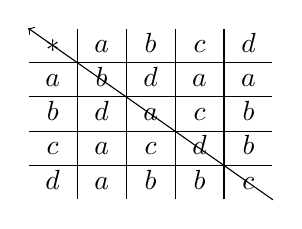
\begin{tikzpicture}\node[inner sep=0pt] (booktable) {
\begin{tabular}{c|c|c|c|c}
\BookInline{\ast } & \BookInline{a} & \BookInline{b} & \BookInline{c} & \BookInline{d}\\\hline
\BookInline{a} & \BookInline{b} & \BookInline{d} & \BookInline{a} & \BookInline{a}\\\hline
\BookInline{b} & \BookInline{d} & \BookInline{a} & \BookInline{c} & \BookInline{b}\\\hline
\BookInline{c} & \BookInline{a} & \BookInline{c} & \BookInline{d} & \BookInline{b}\\\hline
\BookInline{d} & \BookInline{a} & \BookInline{b} & \BookInline{b} & \BookInline{c}\\
\end{tabular}
};\draw[<-] (booktable.north west)--(booktable.south east);\end{tikzpicture}
\end{adjustbox}\end{center}\end{minipage}
\end{center}
\end{BookFloat}

\end{BookBody}

% Source PDF page 33; original printed page 16
\BookSource{33}{16}
\BookNarrativetrue

\begin{BookBody}

\BookLabel{1.24 Example} When an operation has an identity element, it is customary to put the identity first in the list of heads. This makes the first row and the first column match the head row and head column as seen in Table \BookInline{1.25.}\BookEnd{\blacktriangle}

\BookTextHeading{\textbf{Some Words of Warning}  }

\begin{BookFloat}{01_binary_operations-p33-2}
\begin{center}\small\textbf{1.25 Table}\end{center}
\begin{center}\begin{adjustbox}{max width=\linewidth}
\renewcommand{\arraystretch}{1.2}\setlength{\tabcolsep}{5pt}
\begin{tabular}{c|c|c|c|c}
* & \BookInline{e} & \BookInline{a} & \BookInline{b} & \BookInline{c}\\\hline
\BookInline{e} & \BookInline{e} & \BookInline{a} & \BookInline{b} & \BookInline{c}\\\hline
\BookInline{a} & \BookInline{a} & \BookInline{c} & \BookInline{c} & \BookInline{a}\\\hline
\BookInline{b} & \BookInline{b} & \BookInline{a} & \BookInline{e} & \BookInline{c}\\\hline
\BookInline{c} & \BookInline{c} & \BookInline{e} & \BookInline{a} & \BookInline{b}\\
\end{tabular}
\end{adjustbox}\end{center}
\end{BookFloat}

\noindent Classroom experience shows the chaos that may result if a student is given a set and asked to define some binary operation on it. Remember that in an attempt to define a binary operation \BookInline{\ast } on a set S we must be sure that

\BookExercise{1.}{\textit{exactly one element is assigned to each possible ordered pair of elements of} \BookInline{S,\allowbreak }}

\BookExercise{2.}{\textit{for each ordered pair of elements of} \BookInline{S,\allowbreak } \textit{the element assigned to it is again in} \BookInline{S.}}

\noindent Regarding Condition 1, a student will often make an attempt that assigns an element of \BookInline{S} to “most” ordered pairs, but for a few pairs, determines no element. In this event, \BookInline{\ast } is\textbf{ not everywhere defined} on \BookInline{S.} It may also happen that for some pairs, the attempt could assign any of several elements of \BookInline{S,\allowbreak } that is, there is ambiguity. In any case of ambiguity\BookInline{,\allowbreak \ast } is\textbf{ not well defined}. If Condition 2 is violated, then \BookInline{S} is\textbf{ not closed} \textbf{under} \BookInline{\ast.}

\BookLabel{1.26 Example} On which of the sets \BookInline{\mathbb{Q},\allowbreak \mathbb{Q}^{\ast },\allowbreak } and \BookInline{Z^{+ }} does the formula \BookInline{a\ast b= a/b} define an operation? Note that this formula does not make sense in the case that \BookInline{b= 0.} So for example, \BookInline{2\ast 0= 2/0} is not defined, which means Condition 1 is not satisfied. So \BookInline{\ast } is not an operation on \BookInline{\mathbb{Q}.}

If we throw out 0, we do have an operation on \BookInline{\mathbb{Q}^{\ast }} since both Conditions 1 and 2 are satisfied. That is, for any \BookInline{a,\allowbreak b\in \mathbb{Q}^{\ast },\allowbreak a\ast b= a/b} is a nonzero rational number.

The set \BookInline{\mathbb{Z}^{+ }} does not include 0, but there is another issue. For example\BookInline{,\allowbreak 1\ast 2= } \BookInline{1/2\not \in \mathbb{Z}^{+ },\allowbreak } which means that Condition 2 is violated and \BookInline{\ast } is not an operation on \BookInline{\mathbb{Z}^{+ }.}\BookEnd{\blacktriangle}

Following are several illustrations of attempts to define operations on sets. Some of them need some work! The symbol \BookInline{\ast } is used for the attempted operation in all these examples.

\BookLabel{1.27 Example} Let \BookInline{F} be the set of all real-valued functions with domain \BookInline{\mathbb{R}} as in Example 1.7. Suppose we “define” \BookInline{\ast } to give the usual quotient of \BookInline{f} by \BookInline{g,\allowbreak } that is\BookInline{,\allowbreak f\ast g= h,\allowbreak } where \BookInline{h(x)= } \BookInline{f(x)/g(x).} Here Condition 2 is violated, for the functions in \BookInline{F} are defined for\textit{ all} real numbers, and for some \BookInline{g\in F,\allowbreak g(x)} will be zero for some values of \BookInline{x} in \BookInline{\mathbb{R}} and \BookInline{h(x)} would not be defined at those numbers in \BookInline{\mathbb{R}.} For example, if \BookInline{f(x)= } cos \BookInline{x} and \BookInline{g(x)= x^{2},\allowbreak } then \BookInline{h(0)} is undefined, so \BookInline{h\notin F.}\BookEnd{\blacktriangle}

\BookLabel{1.28 Example} Let \BookInline{F} be as in Example 1.27 and let \BookInline{f\ast g= h,\allowbreak } where \BookInline{h} is the function greater than both \BookInline{f} and \BookInline{g.} This “definition” is extremely vague. In the first place, we have not defined what it means for one function to be greater than another. Even if we had, any sensible definition would result in there being many functions greater than both \BookInline{f} and \BookInline{g,\allowbreak } and \BookInline{\ast } would still be\textit{ not well defined}\BookInline{.}\BookEnd{\blacktriangle}

\BookLabel{1.29 Example} Let \BookInline{S} be a set consisting of 20 people, no two of whom are of the same height. Define \BookInline{\ast } by \BookInline{a\ast b= c,\allowbreak } where \BookInline{c} is the tallest person among the 20 in \BookInline{S.} This is a perfectly good binary operation on the set, although not a particularly interesting one\BookInline{.}\BookEnd{\blacktriangle}

\BookLabel{1.30 Example} Let \BookInline{S} be as in Example 1.29 and let \BookInline{a\ast b= c,\allowbreak } where \BookInline{c} is the shortest person in \BookInline{S} who is taller than both \BookInline{a} and \BookInline{b.} This \BookInline{\ast } is\textit{ not everywhere defined,} since if either \BookInline{a} or \BookInline{b} is the tallest person in the set\BookInline{,\allowbreak a\ast b} is not determined\BookInline{.}\BookEnd{\blacktriangle}

\end{BookBody}

% Source PDF page 34; original printed page 17
\BookSource{34}{17}
\BookNarrativefalse

\begin{BookBody}

\BookExerciseTitle{1}

\BookTextHeading{\textbf{Computations}}

\noindent Exercises 1 through 4 concern the binary operation \BookInline{\ast } defined on \BookInline{S= \{a,\allowbreak b,\allowbreak c,\allowbreak d,\allowbreak e\}} by means of Table 1.31.

\BookExercise{1.}{Compute \BookInline{b\ast d,\allowbreak c\ast c,\allowbreak } and \BookInline{[(a\ast c)\ast e]\ast a.}}

\BookExercise{2.}{Compute \BookInline{(a\ast b)\ast c} and \BookInline{a\ast (b\ast c).} Can you say on the basis of this computation whether \BookInline{\ast } is associative?}

\BookExercise{3.}{Compute \BookInline{(b\ast d)\ast c} and \BookInline{b\ast (d\ast c).} Can you say on the basis of this computation whether \BookInline{\ast } is associative?}

\BookExercise{4.}{Is \BookInline{\ast } commutative? Why?}

\BookExercise{5.}{Complete Table 1.32 so as to define a commutative binary operation \BookInline{\ast } on \BookInline{S= \{a,\allowbreak b,\allowbreak c,\allowbreak d\}.}}

\BookExercise{6.}{Table 1.33 can be completed to define an associative binary operation \BookInline{\ast } on \BookInline{S= \{a,\allowbreak b,\allowbreak c,\allowbreak d\}.} Assume this is possible and compute the missing entries. Does \BookInline{S} have an identity element?}

\begin{BookFloat}{01_binary_operations-p34-9}
\begin{center}
\begin{minipage}[t]{0.3135\linewidth}\vspace{0pt}\begin{center}\small\textbf{1.31 Table}\end{center}
\begin{center}\begin{adjustbox}{max width=\linewidth}
\renewcommand{\arraystretch}{1.2}\setlength{\tabcolsep}{5pt}
\begin{tabular}{c|c|c|c|c|c}
* & \BookInline{a} & \BookInline{b} & \BookInline{c} & \BookInline{d} & \BookInline{e}\\\hline
\BookInline{a} & \BookInline{a} & \BookInline{b} & \BookInline{c} & \BookInline{b} & \BookInline{d}\\\hline
\BookInline{b} & \BookInline{b} & \BookInline{c} & \BookInline{a} & \BookInline{e} & \BookInline{c}\\\hline
\BookInline{c} & \BookInline{c} & \BookInline{a} & \BookInline{b} & \BookInline{b} & \BookInline{a}\\\hline
\BookInline{d} & \BookInline{b} & \BookInline{e} & \BookInline{b} & \BookInline{e} & \BookInline{d}\\\hline
\BookInline{e} & \BookInline{d} & \BookInline{b} & \BookInline{a} & \BookInline{d} & \BookInline{c}\\
\end{tabular}
\end{adjustbox}\end{center}\end{minipage}\hfill\begin{minipage}[t]{0.2616\linewidth}\vspace{0pt}\begin{center}\small\textbf{1.32 Table}\end{center}
\begin{center}\begin{adjustbox}{max width=\linewidth}
\renewcommand{\arraystretch}{1.2}\setlength{\tabcolsep}{5pt}
\begin{tabular}{c|c|c|c|c}
* & \BookInline{a} & \BookInline{b} & \BookInline{c} & \BookInline{d}\\\hline
\BookInline{a} & \BookInline{a} & \BookInline{b} & \BookInline{c} & \\\hline
\BookInline{b} & \BookInline{b} & \BookInline{d} &  & \BookInline{c}\\\hline
\BookInline{c} & \BookInline{c} & \BookInline{a} & \BookInline{d} & \BookInline{b}\\\hline
\BookInline{d} & \BookInline{d} &  &  & \BookInline{a}\\
\end{tabular}
\end{adjustbox}\end{center}\end{minipage}\hfill\begin{minipage}[t]{0.2597\linewidth}\vspace{0pt}\begin{center}\small\textbf{1.33 Table}\end{center}
\begin{center}\begin{adjustbox}{max width=\linewidth}
\renewcommand{\arraystretch}{1.2}\setlength{\tabcolsep}{5pt}
\begin{tabular}{c|c|c|c|c}
* & \BookInline{a} & \BookInline{b} & \BookInline{c} & \BookInline{d}\\\hline
\BookInline{a} & \BookInline{a} & \BookInline{b} & \BookInline{c} & \BookInline{d}\\\hline
\BookInline{b} & \BookInline{b} & \BookInline{a} & \BookInline{c} & \BookInline{d}\\\hline
\BookInline{c} & \BookInline{c} & \BookInline{d} & \BookInline{c} & \BookInline{d}\\\hline
\BookInline{d} &  &  &  & \\
\end{tabular}
\end{adjustbox}\end{center}\end{minipage}
\end{center}
\end{BookFloat}

\noindent In Exercises 7 through 11, determine whether the operation \BookInline{\ast } is associative, whether the operation is commutative, and whether the set has an identity element.

\BookExercise{7.}{\BookInline{\ast } defined on \BookInline{\mathbb{Z}} by letting \BookInline{a\ast b= a- b}}

\BookExercise{8.}{\BookInline{\ast } defined on \BookInline{\mathbb{Q}} by letting \BookInline{a\ast b= 2ab+ 3}}

\BookExercise{9.}{\BookInline{\ast } defined on \BookInline{\mathbb{Z}} by letting \BookInline{a\ast b= ab+ a+ b}}

\BookExercise{10.}{\BookInline{\ast } defined on \BookInline{\mathbb{Z}^{+ }} by letting \BookInline{a\ast b= 2^{ab}}}

\BookExercise{11.}{\BookInline{\ast } defined on \BookInline{\mathbb{Z}^{+ }} by letting \BookInline{a\ast b= a^{b}}}

\BookExercise{12.}{Let \BookInline{S} be a set having exactly one element. How many different binary operations can be defined on \BookInline{S}? Answer the question if \BookInline{S} has exactly 2 elements; exactly 3 elements; exactly \BookInline{n} elements.}

\BookExercise{13.}{How many different commutative binary operations can be defined on a set of 2 elements? on a set of 3 elements? on a set of \BookInline{n} elements?}

\BookExercise{14.}{How many different binary operations on a set \BookInline{S} with \BookInline{n} elements have the property that for all \BookInline{x\in S,\allowbreak x\ast x= x}?}

\BookExercise{15.}{How many different binary operations on a set \BookInline{S} with \BookInline{n} elements have an identity element?}

\BookTextHeading{\textbf{Concepts}}

\noindent In Exercises 16 through 19, correct the definition of the italicized term without reference to the text, if correction is needed, so that it is in a form acceptable for publication.

\BookExercise{16.}{A binary operation \BookInline{\ast } is\textit{ commutative} if and only if \BookInline{a\ast b= b\ast a.}}

\BookExercise{17.}{A binary operation \BookInline{\ast } on a set \BookInline{S} is\textit{ associative} if and only if, for all \BookInline{a,\allowbreak b,\allowbreak c\in S,\allowbreak } we have \BookInline{(b\ast c)\ast a= b\ast (c\ast a).}}

\BookExercise{18.}{A subset \BookInline{H} of a set \BookInline{S} is\textit{ closed} under a binary operation \BookInline{\ast } on \BookInline{S} if and only if \BookInline{(a\ast b)\in H} for all \BookInline{a,\allowbreak b\in S.}}

\BookExercise{19.}{An identity in the set \BookInline{S} with operation \BookInline{\ast } is an element \BookInline{e\in S} such that \BookInline{a\ast e= e\ast a= a.}}

\BookExercise{20.}{Is there an example of a set \BookInline{S,\allowbreak } a binary operation on \BookInline{S,\allowbreak } and two different elements \BookInline{e_{1},\allowbreak e_{2}\in S} such that for all \BookInline{a\in S,\allowbreak e_{1}\ast a= a} and \BookInline{a\ast e_{2}= a}? If so, give an example and if not, prove there is not one.}

\end{BookBody}

% Source PDF page 35; original printed page 18
\BookSource{35}{18}
\BookNarrativefalse

\begin{BookBody}

\noindent In Exercises 21 through 26, determine whether the definition of \BookInline{\ast } does give a binary operation on the set. In the event that \BookInline{\ast } is not a binary operation, state whether Condition 1, Condition 2, or both conditions regarding defining binary operations are violated.

\BookExercise{21.}{On \BookInline{\mathbb{Z}^{+ },\allowbreak } define \BookInline{a\ast b= b^{a}.}}

\BookExercise{22.}{On \BookInline{\mathbb{R}^{+ },\allowbreak } define \BookInline{\ast } by letting \BookInline{a\ast b= 2a- b.}}

\BookExercise{23.}{On \BookInline{\mathbb{R}^{+ },\allowbreak } define \BookInline{\ast } by \BookInline{a\ast b} to be the minimum of \BookInline{a} and \BookInline{b- 1} if they are different and their common value if they are the same.}

\BookExercise{24.}{On \BookInline{\mathbb{R},\allowbreak } define \BookInline{a\ast b} to be the number \BookInline{c} so that \BookInline{c^{b}= a.}}

\BookExercise{25.}{On \BookInline{\mathbb{Z}^{+ },\allowbreak } define \BookInline{\ast } by letting \BookInline{a\ast b= c,\allowbreak } where \BookInline{c} is at least 5 more than \BookInline{a+ b.}}

\BookExercise{26.}{On \BookInline{\mathbb{Z}^{+ },\allowbreak } define \BookInline{\ast } by letting \BookInline{a\ast b= c,\allowbreak } where \BookInline{c} is the largest integer less than the product of \BookInline{a} and \BookInline{b.}}

\BookExercise{27.}{Let $H$ be the subset of $M_2(\mathbb{R})$ consisting of all matrices of the form $\begin{bmatrix}a&-b\\b&a\end{bmatrix}$ for $a,b\in\mathbb{R}$. Is $H$ closed under \textbf{a.} matrix addition? \textbf{b.} matrix multiplication?}

\BookExercise{28.}{Determine whether each of the following is true or false.}

\BookExercise{a.}{If \BookInline{\ast } is any binary operation on any set \BookInline{S,\allowbreak } then \BookInline{a\ast a= a} for all \BookInline{a\in S.}}

\BookExercise{b.}{If \BookInline{\ast } is any commutative binary operation on any set \BookInline{S,\allowbreak } then \BookInline{a\ast (b\ast c)= (b\ast c)\ast a} for all \BookInline{a,\allowbreak b,\allowbreak c\in S.}}

\BookExercise{c.}{If \BookInline{\ast } is any associative binary operation on any set \BookInline{S,\allowbreak } then \BookInline{a\ast (b\ast c)= (b\ast c)\ast a} for all \BookInline{a,\allowbreak b,\allowbreak c\in S.}}

\BookExercise{d.}{The only binary operations of any importance are those defined on sets of numbers.}

\BookExercise{e.}{A binary operation \BookInline{\ast } on a set \BookInline{S} is commutative if there exist \BookInline{a,\allowbreak b\in S} such that \BookInline{a\ast b= b\ast a.}}

\BookExercise{f.}{Every binary operation defined on a set having exactly one element is both commutative and associative.}

\BookExercise{g.}{A binary operation on a set \BookInline{S} assigns at least one element of \BookInline{S} to each ordered pair of elements of \BookInline{S.}}

\BookExercise{h.}{A binary operation on a set \BookInline{S} assigns at most one element of \BookInline{S} to each ordered pair of elements of \BookInline{S.}}

\BookExercise{i.}{A binary operation on a set \BookInline{S} assigns exactly one element of \BookInline{S} to each ordered pair of elements of \BookInline{S.}}

\BookExercise{j.}{A binary operation on a set \BookInline{S} may assign more than one element of \BookInline{S} to some ordered pair of elements of \BookInline{S.}}

\BookExercise{k.}{For any binary operation \BookInline{\ast } on the set \BookInline{S,\allowbreak } if \BookInline{a,\allowbreak b,\allowbreak c\in S} and \BookInline{a\ast b= a\ast c,\allowbreak } then \BookInline{b= c.}}

\BookExercise{l.}{For any binary operation \BookInline{\ast } on the set \BookInline{S,\allowbreak } there is an element \BookInline{e\in S} such that for all \BookInline{x\in S,\allowbreak x\ast e= x.}}

\BookExercise{m.}{There is an operation on the set \BookInline{S= \{e_{1},\allowbreak e_{2},\allowbreak a\}} so that for all \BookInline{x\in S,\allowbreak e_{1}\ast x= e_{2}\ast x= x.}}

\BookExercise{n.}{Identity elements are always called \BookInline{e.}}

\BookExercise{29.}{Give a set different from any of those described in the examples of the text and not a set of numbers. Define two different binary operations \BookInline{\ast } and \BookInline{\ast ^{\prime }} on this set. Be sure that your set is\textit{ well defined}.}

\BookTextHeading{\textbf{Theory}}

\BookExercise{30.}{Prove that if \BookInline{\ast } is an associative and commutative binary operation on a set \BookInline{S,\allowbreak } then}

\begin{center}\begin{adjustbox}{max width=\linewidth}\BookInline{\displaystyle (a\ast b)\ast (c\ast d)= [(d\ast c)\ast a]\ast b}\end{adjustbox}\end{center}

\noindent for all \BookInline{a,\allowbreak b,\allowbreak c,\allowbreak d\in S.} Assume the associative law only for triples as in the definition, that is, assume only

\begin{center}\begin{adjustbox}{max width=\linewidth}\BookInline{\displaystyle (x\ast y)\ast z= x\ast (y\ast z)}\end{adjustbox}\end{center}

\noindent for all \BookInline{x,\allowbreak y,\allowbreak z\in S.}

\noindent In Exercises 31 and 32, either prove the statement or give a counterexample.

\BookExercise{31.}{Every binary operation on a set consisting of a single element is both commutative and associative.}

\BookExercise{32.}{Every commutative binary operation on a set having just two elements is associative.}

\noindent Let \BookInline{F} be the set of all real-valued functions having as domain the set \BookInline{\mathbb{R}} of all real numbers. Example 1.7 defined the binary operations \BookInline{+,\allowbreak -,\allowbreak \cdot,\allowbreak } and \BookInline{\circ } on \BookInline{F.} In Exercises 33 through 41, either prove the given statement or give a counterexample.

\BookExercise{33.}{Function addition \BookInline{+ } on \BookInline{F} is associative.}

\BookExercise{34.}{Function subtraction \BookInline{- } on \BookInline{F} is commutative.}

\end{BookBody}

% Continuation on source PDF page 36, preceding Section 2
\BookNarrativefalse

\begin{BookBody}

\BookExercise{35.}{Function subtraction \BookInline{- } on \BookInline{F} is associative.}

\BookExercise{36.}{Under function subtraction \BookInline{- F} has an identity.}

\BookExercise{37.}{Under function multiplication \BookInline{\cdot F} has an identity.}

\BookExercise{38.}{Function multiplication \BookInline{\cdot } on \BookInline{F} is commutative.}

\BookExercise{39.}{Function multiplication \BookInline{\cdot } on \BookInline{F} is associative.}

\BookExercise{40.}{Function composition \BookInline{\circ } on \BookInline{F} is commutative.}

\BookExercise{41.}{If \BookInline{\ast } and \BookInline{\ast ^{\prime }} are any two binary operations on a set \BookInline{S,\allowbreak } then}

\begin{center}\begin{adjustbox}{max width=\linewidth}\BookInline{\displaystyle a\ast (b\ast ^{\prime }c)= (a\ast b)\ast ^{\prime }(a\ast c)\;\text{for all}\;a,\allowbreak b,\allowbreak c\in S.}\end{adjustbox}\end{center}

\BookExercise{42.}{Suppose that \BookInline{\ast } is an\textit{ associative binary} operation on a set \BookInline{S.} Let \BookInline{H= \{a\in S\mid a\ast x= x\ast a} for all \BookInline{x\in S\}.} Show that \BookInline{H} is closed under \BookInline{\ast.(}We think of \BookInline{H} as consisting of all elements of \BookInline{S} that\textit{ commute} with every element in \BookInline{S.)}}

\BookExercise{43.}{Suppose that \BookInline{\ast } is an associative and commutative binary operation on a set \BookInline{S.} Show that \BookInline{H= \{a\in S\mid a\ast a= } \BookInline{a\}} is closed under \BookInline{\ast.(}The elements of \BookInline{H} are\textbf{ idempotents} of the binary operation \BookInline{\ast.)}}

\BookExercise{44.}{Let \BookInline{S} be a set and let \BookInline{\ast } be a binary operation on \BookInline{S} satisfying the two laws}

\BookBullet{\BookInline{x\ast x= x} for all \BookInline{s\in S,\allowbreak } and}

\BookBullet{\BookInline{(x\ast y)\ast z= (y\ast z)\ast x} for all \BookInline{x,\allowbreak y,\allowbreak z\in S.}}

Show that \BookInline{\ast } is associative and commutative. (This is problem B-1 on the 1971 Putnam Competition.)

\end{BookBody}
\ifdefined\BookMaster\let\BookFinish\relax\else\def\BookFinish{\end{document}}\fi\BookFinish
